
%\newcommand{\root}{Chapters/face}

\chapter{Getting Off the Internet: Practical Domain Adaptation for Face Recognition}
\label{chapt:wildface_}


\section{Motivation}
%face
For face recognition, one important cross-domain scenario is related to using powerful models pretrained on professional photographs for surveillance data. As it has been already mentioned in \sect{face}, large-scale training datasets for face recognition most often include high-quality images that are very different from those captured by surveillance systems. In person re-identification, the domain difference comes mainly from the illumination condition variations between the camera sets (if the difference of the camera positions is put aside). In contrast,  surveillance face recognition implies a complex domain shift caused by a combination of low resolution, compression and illumination conditions. 


In particular, in this chapter we study the unsupervised domain adaptation scenario, where face recognition is trained using an annotated Internet face dataset and an unannotated dataset of faces collected from a surveillance camera network with low image quality. We mostly focus on the recent class of methods that consider domain-adaptation at the image level. We thus investigate how image transformation achieved with recent unsupervised image transformation techniques such as CycleGAN (\cite{ZhuPIE17}) can be used for face recognition under strong domain shifts. 

We compare and evaluate several strategies, such as transferring test data to the Internet image domain,  transferring training data to the target domain followed by retraining the network. As a baseline, we also compare to adversarial domain adaptation at feature level described in \chapt{gradrev}.% \cite{GaninUAGLLML16}. 

Our comparison suggests that image transformation (without explicit modeling of separate degradation factors) can be used for unsupervised domain adaptation of face recognition. We, however, demonstrate that special care needs to be taken in order to make such domain adaptation work better than baselines, and come up with practical suggestions on how such improvement can be achieved.

%model
% Since the CycleGAN \cite{cyclegan} architecture for image-to-image translation and stylization appeared, domain adaptation has become one of its active fields of application. This approach differs from the feature-level domain adaptation techniques of \cite{LongC0J15} and \cite{tzeng2014deep} or the method presented in the \chapt{gradrev}, because rather than finding deep domain-invariant representations, it works on the pixel level and aims at building mappings between the image domains. Thus the domain adaptation is done in two steps: building a mapping the source domain to target and retraining the predictor on the transferred source data. (Although it is also possible to combine these two steps into one optimization process.)%cycada

% %pedestrians
% For person re-identification, the pixel-level domain adaptation with CycleGAN has been applied in several recent works \cite{} (after the results of the \chapt{gradrev} were published). Some of them consider different datasets as domains, others aim at utilising synthetic re-identification data to improve the results on real data \cite{}. As demonstrated by these works, image-to-image translation may help a lot to overcome the illumination differences between the source and target camera sets. %Still, to the best of our knowledge, there are no works approaching face recognition for surveillance data.

% This chapter demonstrates the performance of the pixel-level domain adaptation approach based on CycleGAN model in the presence of an extreme domain shift between the usual face recognition training data and surveillance data. The considered surveillance data are harvested from $6$ surveillance cameras in the Moscow subway. Two publicly available face recognition datasets of different image quality are considered for the source domain. The approach is compared to several important baselines, including the reverse translation of the target images back to the source domain and the feature-level domain adaptation suggested in this chapter.

%The remainder of the chapter is organized as follows. Image-level domain transfer and face recognition methods are described in \sect{method}.  We define the variants of the training data augmentation compared in this work in \sect{ft}. Then we give the implementation details in \sect{training}. The quantitative comparisons of the described methods and baselines are presented in \sect{results}. Finally, we conclude the work with discussion and summary in \sect{conclusion}.



%\titlerunning{Short form of title}        % if too long for running head



% \begin{abstract}
% Face recognition in real surveillance scenarios is challenging due to the presence of complex degradation factors. At the same time, the easiest-to-collect and the biggest available training data for face recognition come from the Internet, where images and video frames have higher quality, higher resolution, and better lighting. In this work, we study training face recognition systems under such domain shift. We show that CycleGAN technique can be utilized for transferring labeled training data into the target domain of surveillance camera, and that the transferred data can be used to train face recognition in the new domain. We compare this approach to several baselines including the domain transfer in the opposite direction to turn test data directly to the high-quality domain. Our comparison and evaluation allow us to come up with a viable strategy for training face recognition in surveillance data.
% \keywords{face recognition \and surveillance \and domain adaptation}
% % \PACS{PACS code1 \and PACS code2 \and more}
% % \subclass{MSC code1 \and MSC code2 \and more}
% \end{abstract}


%% !TEX root = ../Thesis_main.tex
\chapter{Introduction}

%video surveillance+
%person re-id+
% originates from Multi-Target Multi-Camera Tracking 
%open world / closed world+
%face : verification/identification
%common aspects: detection , processing, recognition
%deep learning

%retrieval
%fine-grained recognition
%adaptation

%datasets (cut from the papers) + table with reid dataset?
%architectures
%definitions?
%contribution - what is done
\section{Context}
\subsection{Problem of 3D reconstruction}

\subsection{Approaches for solving 3D Reconstruction problem}

Solutions for a reconstruction problem can be grouped in two major groups: 1) Geometric approach - when problem is represented as optimisation of scene state given constrains on projections of scene state to data, 2) Machine Learning approach - inverse model is optimisation.

If $X$ - is scene data, $z$ - is the state of the scene, and $g_i(z)$ - projection function of 3D scene $z$ state to perspective $i$, then to find an optimal 3D reconstruction, one solves this minimisation problem:
\begin{equation}
z_{rec} = \min_z\sum_i|X_i-g_i(z)|_2 .
\end{equation}

This approach only solves problem for once scene and does not provide any semantic information about it, only basic geometric information. 
The second approach is more modern and better fitted for machine learning applications, because instead of optimizing state of the scene, it's optimizes a model that performs computation from input data to some semantic (intrinsic) parameters, and can be described as following optimisation procedure:
\begin{equation}
\min_\theta\sum_i|X_i-g_i(f_\theta(\pi))|_2,\ \ \pi=I_\theta(\{X_i\}_i),\ \ z=f_\theta(\pi),
\end{equation}
where $\pi$ - are scene parameters, $f_\theta(\pi)$ - is a generative model that generates 3D state $z$ and it's function is determined by tunable parameters $\theta$.

In reconstruction process information can be introduced in two possible ways: 1) input signal - data measured by some spatial sensor, 2) by adding a priori knowledge while training the Inverse model or by design choice of reconstruction algprithm. Between the two source exist a fundamental trade-off and detirmination of which is dominant can be quite difficult \cite{tatarchenko2019single}.


\subsection{Objectives and Motivations}

The goal of this work to improve methods of 3D reconstruction in holistic context using deep learning systems. For efficient applications such as robotics in human environments and mixed reality more advanced machine perception systems are needed. Human perception is a complex system with several properties not all of which are replicated in modern machine perception systems. From cognitive sciences it's known that ability to model environments is one of the most important for perception system, in area of computer vision this is known as an ability to perform \textit{3D reconstruction} of scenes and environments. To solve this problem in a general case requires application of machine learning.

In particular, the development of such holistic deep 3D reconstruction system includes several important tasks:

\begin{itemize}
􏰀    \item Capturing scenes, complete with colour and depth data of a sufficient quality,
    \item Recalling objects from large scale database of objects,
    \item Segmenting variety of most common elements from sensor data, such as household objects and architectural components,
    \item Detecting and reconstructing shape and pose of and human bodies.
\end{itemize}

Each of these sub-tasks constitutes a challenge in the context of human perception.

The presence of noise in sensor data (e.g., consumer grade depth cameras) is a serious problem for all downstream sub-tasks, low fidelity of this data causes a considerable compaunding performance drop.

\subsection{3D data representations}

We can describe a 3D object in multiple ways, and codification of it's properties has ramifications about capturing different information about objects and scenes, as well as kinds of models that can regenerate them or computational resources needed to process it.
Each representation has it's own pros and cons. We assume 3D information representation to be positive effective and usefull if it captures more relevant information with less storage requirement (compression), increases signal to noise ratio of data, captures shape and texture properties with minimum trade-off.

Here are some popular examples of 3D data representations:
\begin{enumerate}
	\item Multiple 2D projections - captures surface texture, highly redundant representation if images overlap, also vulnerable to optic illusions.
	\item Voxels - simple, most of the time can be sparse, represents rough volumetric properties vell but losses most of surface properties.
	\item Point Cloud - are sparse in a sense that they don't capture empty space, losing all surface properties besides color and estimated normals and most of volumetric properties.
	\item 2.5D (RGB-D) images are widespread because of cheap measurement devices, capture volumentric depth but succeptable to occlusion of bodies in a scene and records a lot of noise with actual signal.
\end{enumerate}



%Motivation: RGB-D scanning is here and we want to have a fine-grained understanding of the 3D captures
In the recent years, a wide variety of consumer-grade RGB-D sensors, such as the Intel Real Sense, Microsoft Kinect, depth-sensor enabled smartphones, enabled inexpensive and rapid RGB-D data acquisition. Increasing availability of large, labeled datasets (e.g.,~\cite{chang2017matterport3d,dai2017scannet})  made possible development of deep learning methods for 3D object classification and semantic segmentation. At the same time, acquired 3D data is often incomplete and noisy; while one can identify and segment the objects in the scene, reconstructing high-quality geometry of objects remains a challenging problem.  

An example of the new approach in recent work 
\cite{avetisyan2019scan2cad}, uses a large dataset of clean, labeled geometric shapes
\cite{chang2015shapenet}, for classification/segmentation associating the input point or voxel data with object labels from the dataset, along with adapting geometry to 3D data.  This approach ensures that the output geometry has high quality, and is robust with respect to noise and missing data in the input.  
At the same time, a ``flat'' classification/segmentation approach, with each object in the database corresponding to a separate label and matched to a subpart of the input data corresponding to the whole object, does not scale well as the number of classes grows and often runs into difficulties in the cases of extreme occlusion (only a relatively small part of an object is visible). 
Significant improvements can be achieved by considering object \emph{parts}, or more generally part hierarchies. 
Part-based segmentation of 3D datasets promises to offer a significant improvement both in finding the best matching shape in the dataset, recognizing objects from  highly incomplete data (e.g., from a couple of parts) from  as well as more precise geometry adaptation as well as, potentially, assembly of new shapes out of existing parts yielding a closer match to the input data. 

large collection of 3D models in database can be reduced to structured representations, 
objects with occluded sub-parts still can be recognized by parts available in the scan and the rest can be guessed with high probability, using parts, we can reconstruct new objects that are not yet present in the database of shapes.

Based on different approaches for volumetric information integration, from enhancements of  methods such as volumetric fusion \cite{curless1996volumetric}, to probabilistic  methods, and plethora of methods based on their combinations.

Compared to computer graphics models manually created by 3D professionals, 3D scans are noisy and incomplete.
Amount of noise and limited resolution of consumer-grade scanning hardware pose significant challenges for solving this important problem of scene reconstruction. 
Approaches of reconstruction based on fitting existing 3D assets into scene scans, have shown a lot of promise but still had problems with finding exact models from large database such as ShapeNet \cite{chang2015shapenet}, because of occlusion and lack of spatial context.

Learning-based approaches are very good at extracting features representative of objects and scenes as a whole, allowing to fill in occluded areas or guess parts affected by noise \cite{dai2017shape,dai2018scancomplete,song2017semantic}. These features are sufficient for scene completion, but they are not as good at recovering geometric primitives like: sharp edges, planar surfaces or borders between sub-parts, resulting in reconstruction quality much poorer than that of 3D content created by humans.

In this work, we focus on the key problem of semantic part segmentation of objects in the scenes, enabling further improvements in  dataset-based reconstruction. 
Semantic part-segmentation, can help in these situations, when sufficient number of the object parts is visible model can infer the non-visible parts essentially completing an object in sense of maximum probability conditioned on input data.

In human-made environments, a lot of objects have naturally defined semantic sub-parts, and those sub-parts can, in turn, have their sub-parts, i.e., parts form \emph{hierarchies}.  In our work, we use scene and object representation based on such part hierarchies.  We show how a part-labeled dataset of scanned 3D data suitable for machine learning applications can be constructed, and used to improve the performance of segmentation algorithms. 

Definitions of sub-parts are based on a set of primitive elements that were manufactured by one formation method or from one material.

Because of that and the fact that static scenes have other relationships between objects (fixed to each other or in direct surface contact), it's reasonable to suggest a scene description format that possesses a property of hierarchy (e.g., trees or other kinds of graphs).
Representing scenes as a discrete structures with multiple relationships between nodes. Such relationships like composability of its parts and affordances between whole objects, in turn allowing to compose a scene from separate objects.

\todo{merge these paragraphs}

In domain of human-made environments a lot of objects have sub-parts and those sub-parts can in turn have their own sub-parts. Definition of sub-part is often based on a set of primitive elements that were manufactured by one formation method or from one material. Because of that and the fact that static scenes have other relationships between objects (fixed to each other or in direct surface contact), it's reasonable to suggest a scene description format that possess a property of hierarchy (e.g. trees or other subgraphs).
A lot of researchers over the last 20 years came to the same conclusion. A lot of work on that problem was done by Mumford and Zhu in \cite{zhu2006stochastic}.

One of the papers dealt with problem of modeling Images as a hierarchy of super-pixels. \cite{russell2009associative}, or as a tree of geometric primitives (e.g. cylinders, spheres or 3D boxes) \cite{li2017grass}.

% point cloud (PC) turned in to a graph (based on proximity) point-cloud parser network reduces number of nodes and edges and enriches their feature vectors. First part of the decoder network functions similar to Feature Pyramid Network in CNNs, which performs local computations on different scales, followed by "pooling or convolutions" with reduced spatial component and increased feature components, thus leaving only small number of "keypoints" required to outline shapes of objects.



CAD constructor network translates that graph into CAD object (tree with primitives and combination rules). CAD rendered makes a mesh out of that object thus a residual between original PC and Mesh can be calculated.

Proximity Graphs - concept that allows to build a bridge between Point Clouds and Graph Processing. This area of computational geometry has a lot of theoretical results to offer for Deep Learning piplene designer.


\subsection{Definitions and examples}
\subsection{Data sources and devices}

\section{Inverse Graphics Problem formulation}

\cite{rezende2016unsupervised,eslami2016attend,kulkarni2015deep,wu20153d,izadinia2017im2cad}

Inverse graphics approach enables to solve a problem of "real-world" scene understanding through reconstruction of that scene and comparison it to measured data in some form.

Because it's a fairly new method it has some unexplored facets:
\begin{enumerate}
    \item How can we scale to hundreds and thousands of objects with different parameters.
    \item Embedded representations better than procedural generation
    \item Are there format that can have all advantages of CAD models and probabilistic properties that arise from real-world uncertainties.
\end{enumerate}

Central goals of computational perception is to get structured description of scenes from measurements such as photographic images, scans and videos.

Computer Vision as Inverse Graphics is the most rational formulations that could help us achieve this goal.

In the past, it has been hard to directly solve these problems in practice because of computational limitations.

However, it may be right time to take another look at this idea due to significant advances in deep learning for computer vision, probabilistic programming, and computer graphics.

Probabilistic programming - a tool that allows us to implement complex models while keeping ability to perform inference, extend with other probabilistic models by being general-purpose.

Re-formalizing inverse graphics in terms of probabilistic programming and deep learning allow us to solve even more complicated vision problems with off-the-shelf computational technology.

To make this approach scalable, my research can incorporate effective techniques such as: approximate Bayesian computation, differentiable programming for rendering.

Computer Graphics nowadays seems to be improving at a great pace in terms of designing solutions for hard image synthesis problems, but these solutions are usually hand-made and not flexible enough to cover all needs for general-purpose real world object generating, latest advances in generative models can help with that.


\subsection{Overcoming lack of information}

\section{Datasets}

Only recently research community started accumuulating sugnifficant amount of algined sensor data to solve large scale 3D reconstruction problems in deep learning context. In last 4 years we saw an explosion of 3D shape databases and 2D-to-3D indoor scene datasets, such as ShapeNet, 2D-3D Semantic, Scannet and Matterport3D datasets. Because accuracy and reacall properties of deep learning models scale with amount and variety of data, number of state-of-the-art models grew as well.

\section{Architectures}

PanopticFusion~\cite{narita2019panopticfusion} is a model that is able to segment large indoor scenes and separate \textit{Stuff} and \textit{Things}.


For outdoor datasets Point Cloud representation of data is more common because of large empty spaces and the way LiDAR sensor collects data. In such setting instance segmentation is nessesary first step for reconstruction~\cite{zhang2020instance}.

\subsection{Multi-view models}

Detailed comparision of multi-view 2D CNN model and 3D volumetric CNN can be found in \cite{qi2016volumetric}.

\subsection{Implicit 2D models}

Like inverse graphics network. Model takes 2D images and returns 2D images with 3D properties changed. 

\subsection{3D convolutional models}

Model generates or processes voxel image with 3D convolutional operation implemented Dense or Sparse.

Semantic information can boost the reconstruction performance because deep learning systems are able to pick up onto consistent signal \cite{jiao2018look,tatarchenko2019single,kendall2018multi}.

\subsection{2D to 3D Projection models}

Model uses camera parameters to compute 3D representation using 2D/2.5D images and projection operation.

\subsection{Point Set layers}

Neural Network processes a set of points to classify, segment or predict new set of points.

\subsection{Graph-Convolutional layers}

Model processes Geometric Graph where nodes represent points registered on a surface of objects or parts of objects, and has geometric or other information representing edges between points. Layers process activations associated with nodes taking into account the connectivity.

\subsection{Differentiable rendering layers}

Rendering operation is implemented in a differentiable way, allowing backpropogation of gradient information from 2D images to meshes and textures of the objects being rendered.

\subsection{Mesh generating layers}

Neaural Network layers that can create a mesh by way of processing a template 3D shape with parametracised operation or meshing other 3D shape representation generated by computation from weights and input.

\subsection{Implicit 3D models}

Models like NeRF, PIFU3D, neural network implements a rendering function depending on view angle and other graphics parameters, one model represents one scene and don't generalise for viriety of scene inputs.



\section{Contributions}

% \chapt{hist}, \chapt{bilinear} and \chapt{gradrev} use  person re-identification architecture of \citep{Yi14} as a baseline method (it is also  described in \sect{intro_architectures}).  \chapt{bilinear} is based on the results of \chapt{hist}: the loss function introduced in \chapt{hist} is used for 
% all the experiments in \chapt{bilinear} as it was demonstrated to show the best performance for person re-identification. 
% The results of \chapt{gradrev} were chronologically the earliest among all the results presented in this work, therefore  methods  from \chapt{hist} and \chapt{bilinear} were not used there. 
% Although the contributions of each of the chapters are independent, they are all parts of building a person re-identification pipeline and can be applied simultaneously. 
% \chapt{wildface} considers domain adaptation for surveillance face recognition and uses the method from \chapt{gradrev} as one of the baselines.
 


 \begin{figure}
 \centering
    \includegraphics[height=0.7\paperheight]{Chapters/face/da_picture_vertical_TS.pdf}
    \caption{The overall scheme of the two possible approaches to the face recognition problem considered in our work. Surveillance and Internet image domains are denoted with green and blue rectangles correspondingly (the data examples are taken from our surveillance dataset and the Youtube faces dataset).
    The \textit{face restoration} approach (blue lines) transfers the surveillance data images to the Internet domain using the transform $F^{T \rightarrow S}$. It then uses the ``blue'' face recognition model trained on annotated internet images to compute descriptors for the transfered images. Meanwhile, the \textit{domain adaptation} approach (green lines) transfers the annotated internet data to the surveillance domain, and then uses the transfered data to train the ``green'' face recognition model, which is then applied to unannotated surveillance images. Our work evaluates and compares several variants of both approaches.}
  \end{figure}

  
%\section{Related work}
\label{sect:related}

There are two main research directions dedicated to face recognition for low-quality data: (i) the face restoration approach and (ii) the domain adaptation approach. In the face restoration-based approach, low-quality images are enhanced and restored to facilitate recognition. The ability to reuse existing recognition systems that were developed for high-quality data comes as a natural benefit of such methods. Domain adaptation methods are conversely aimed to change the existing recognition systems so that they are better suited for the target domain (i.e.\ low resolution/quality images). We now provide a brief review of both approaches.

\subsection{Face restoration methods}

There is a vast range of methods that perform face restoration. In most of them, different degradation types are considered separately. Pan \textit{et al.} \cite{pan2014deblurring} propose an effective face deblurring method based on approximating blur kernel followed by non-blind deconvolution. The blur kernel  approximation is guided by the known non-blurred exemplar with the structure similar to the input image structure. 

In Zhang \textit{et al.}~\cite{ZhangYZNH11}, deblurring and recognition tasks are considered simultaneously. They use a sparse representation of the input image in terms of the gallery image set. The blur kernel and representation coefficients are estimated iteratively. Classification is finally performed based on the classes with the highest coefficients in the sparse representation.  


A number of recent methods \cite{TuzelTH16,ZhuLLT16,xu2017learning,huang2017wavelet} explore the task of restoration of extremely low-resolution images using deep neural networks. All these works utilize the paired (aligned) learning scheme, where the high-resolution ground truth is known for every low-resolution image in the training set. The low-resolution training data are simulated using synthetic degradation of the initial high-resolution images. In \cite{xu2017learning} and \cite{TuzelTH16}, a generative adversarial network~(GAN)~\cite{goodfellow2014generative} is used to force the restoration network to produce more natural images. In \cite{huang2017wavelet}, an additional structure-based loss that uses wavelet transform is suggested for the same goal. While the results of these methods are impressive, there is no direct way to use the paired learning approaches for the arbitrary combination of degradation factors that one may encounter when analyzing real images captured by surveillance cameras. 

\subsection{Domain adaptation methods}

Several recent works are dedicated to domain adaptation in the context of different recognition tasks \cite{Volpi_2018_CVPR,Hong_2018_CVPR,Deng_2018_CVPR,Bousmalis_2017_CVPR,Murez_2018_CVPR}. In \cite{Murez_2018_CVPR}, 
\cite{Bousmalis_2017_CVPR} and \cite{Deng_2018_CVPR}, image-level domain adaptation is performed for segmentation, classification and similarity learning (person re-identification) correspondingly. Hong \textit{et al.} \cite{Hong_2018_CVPR} and Volpi \textit{et al.} \cite{Volpi_2018_CVPR} resort to feature-level domain adaptation for segmentation and classfication tasks. Both feature-level and image-level techniques are used in \cite{Hoffman17}.

Some of the aforementioned methods \cite{Hoffman17,Deng_2018_CVPR,Murez_2018_CVPR} employ CycleGAN framework  to change the domain of training data for classification, segmentation, and person re-identification. Here we explore a similar approach for the task of face recognition in the presence of complex degradation factors.

Hong \textit{et al.} \cite{HongIRY17} and
Sohn \textit{et al.} \cite{SohnLZY0C17} approach face recognition tasks for low-quality image domain. They consider image degradation as a domain shift and perform feature-level unsupervised domain adaptation based on adversarial learning showing better recognition results. 
The works \cite{HongIRY17} and \cite{SohnLZY0C17} are very related to ours: the authors show that domain-specific data augmentation is essential for training face recognition systems. 
 However, in both works, the data augmentation is performed 'by hand' (the degradation types and hyper-parameters for transforms are chosen and fixed), while we augment the training data in an automatic manner utilizing the CycleGAN framework, which can also be viewed as an image-level domain adaptation.
%Additionally, in contrast to \cite{HongIRY17}, we do not consider extremely large pose variation. Instead, we are more focused on the image degradation factors (e.g. the combination of small size, blur, JPEG-compression). 
Differently from \cite{SohnLZY0C17}, where evaluation is performed for the Youtube faces dataset, we approach the task in the presence of the somewhat stronger domain shift, as our test data are captured by surveillance cameras and are mostly of much lower quality.




%Some works already successfully use CycleGAN technique to perform an unsupervised domain adaptation. \cite{CYCADA} approached semantic segmentation. % add avput CYCADA

%recognition and reconstruction approaches
% Several existing works consider restoration and recognition problems jointly. In some works, authors apply the recognition-based priors to achieve better restoration results. \cite{TODO , Xu} 

% There are also approaches jointly performing explicit recognition and restoration
% In \cite{TODO Close  the  loop:  Jointblind  image  restoration  and  recognition  with sparse representation prior , Baker} The  proposed  approaches  perform  recognition  using  a  limited  number  of  gallery  images.   In parallel, they reconstruct the input image and classify it based on labels of the most relevant examples found in the train set.

 
% One of the baselines used in this work applies the similar scheme: CycleGAN framework is used to transfer the low-quality test data into the high-quality domain, the domain classifier serves as 'restoration' loss. We additionally introduce the recognition component into this scheme: another baseline is the same CycleGAN but with domain classifier based that is learned using features calculated with the pre-trained face recognition network.




    \begin{figure}
    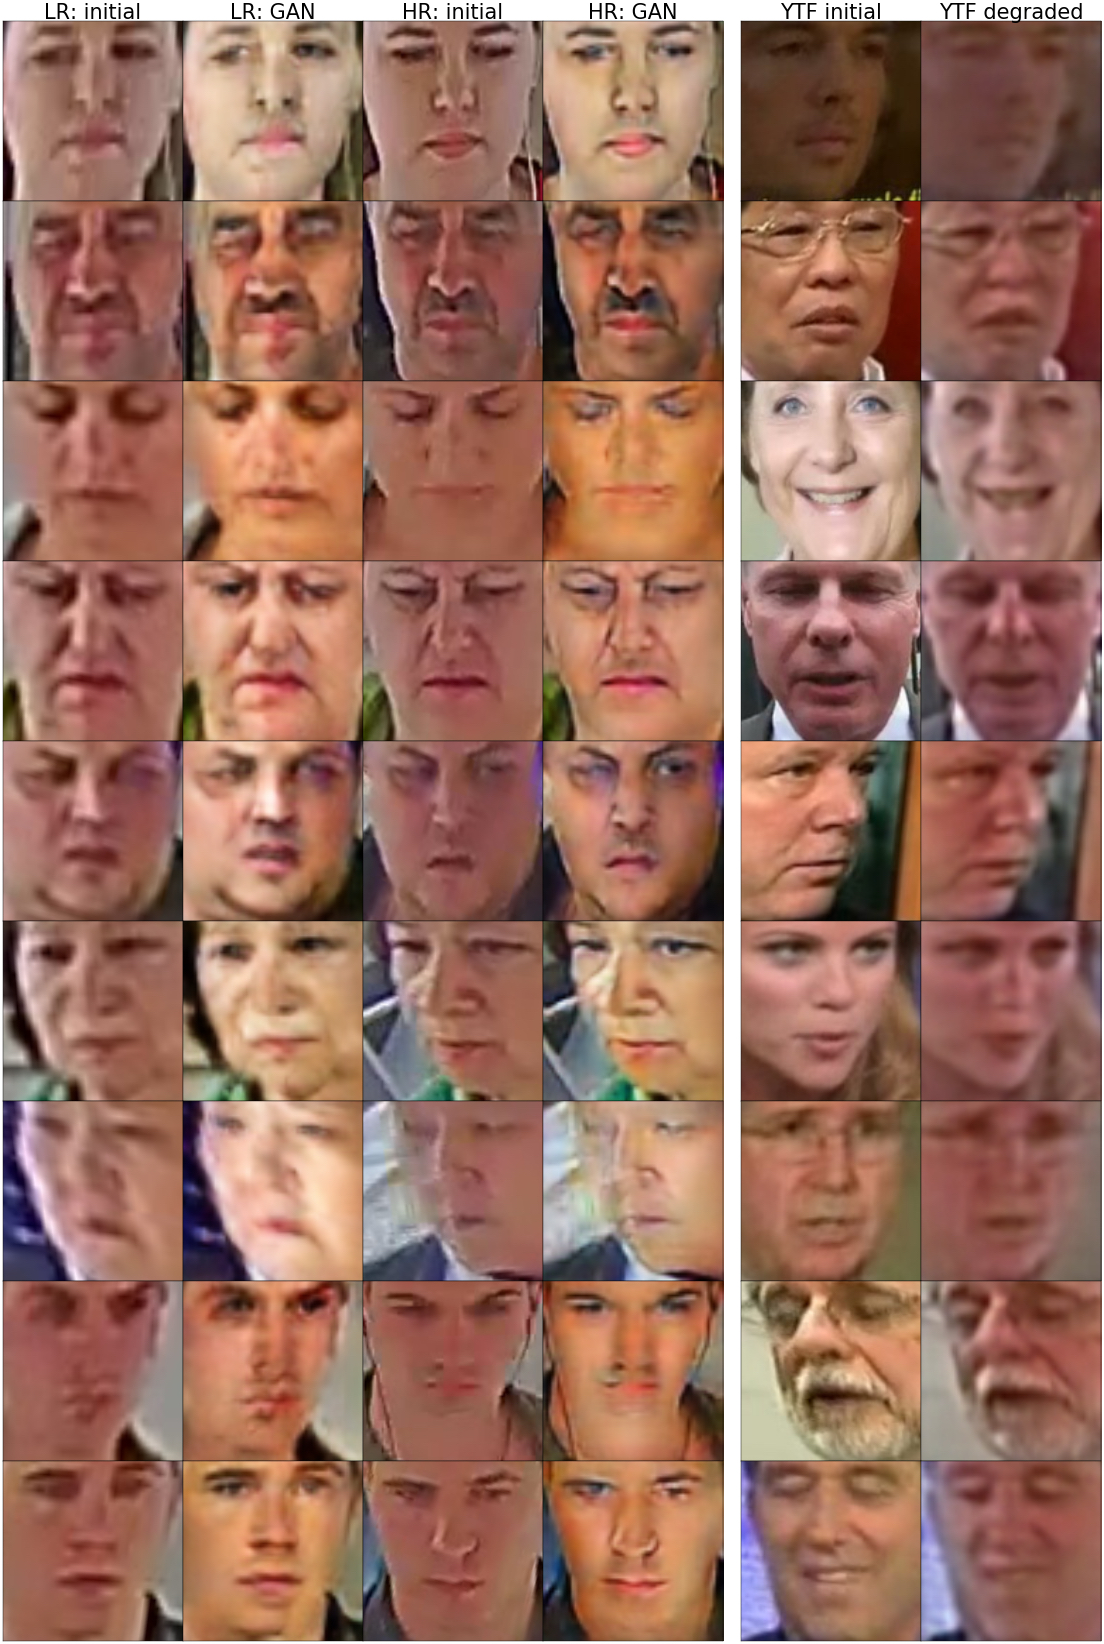
\includegraphics[width=\linewidth]{Chapters/face/Fig2.jpg}
    \caption{Columns one and three show images from our test surveillance data, while columns two and four contain the corresponding images transformed to the Internet data domain. See section \ref{sect:method} for the details. The last two rows show the examples of the reverse transformation from the Internet image domain to the surveillance image domain for the Youtube faces dataset.  }\label{fig:lr_hr_gan_res_ytube_initial_degraded}
  \end{figure}
  
  
\section{Evaluated approaches}
\label{sect:method}
\bigskip
\indent\textbf{Face recognition for the low-quality image domain}\\
%\subsubsection{Face recognition for the low-quality image domain}
\label{sect:strategies}
In this work we consider and compare two main approaches to face recognition for surveillance data: 1) restoration-based approach and 2) domain adaptation of existing face recognition neural networks. 

We consider two facial image domains: \begin{itemize}
\item domain $T: \{X^{T}_{i} \}_{i=0}^{N_T}$ that includes low-quality facial images $X^{T}_{i}$ captured using surveillance cameras. Usually, there are no identity labels provided, as assigning identity labels is quite challenging and may not even be feasible.
\item domain $S: \{(X^{S}_{i}, Y^{S}_{i})\}_{i=0}^{N_S}$ that includes facial images $X^{S}_{i}$ harvested from the Internet. These images are usually of higher quality and are taken in good lighting conditions. We assume that the data in this domain are supplied with identity labels $Y_i$.
\end{itemize}  

According to the available labeling, we can consider two different pipelines for building face recognition systems for surveillance data. The first option is the restoration-based approach when we use transform $F^{T \rightarrow S}: T \longrightarrow S$ as a face restoration method and then apply existing recognition neural network $R^{S}$ that is pre-trained on images from the domain $S$. The second option is to use the transform $F^{S \rightarrow T}: S \longrightarrow T$ to transfer the large collections of labeled training data to the target domain of surveillance images. In this scenario, we retrain the existing face recognition networks resulting in the new adapted model $R^{T}$.

More formally, we consider the following two pipelines for face recognition in the domain $T$.  We denote $d^{T}$ and $d^{S}$ the descriptors produced by the domain-specific face recognition models $R^{T}$ and $R^{S}$. These descriptors may be used e.g.\ to identify matching and non-matching faces based on the distances between them. 
 
$F^{T \rightarrow S}: T \longrightarrow S$ and $F^{S \rightarrow T}: B \longrightarrow A$ are the image-level domain transfer mappings. In the restoration-based approach, we train the recognition model $R^{S}$ using labeled data  $\{(X^{S}_{i}, Y^{S}_{i})\}$ where $X^{S}_{i} \subseteq B$. We then test the learned model by computing the descriptors $d^{S}$ after applying the network $F^{T \rightarrow S}$:  $d^{S} = R^{S}(X^{T\rightarrow S}) = R^{S}(F^{T \rightarrow S}(X^{T}))$

In the domain adaptation approach, we train the recognition network $R^{T}$ using labeled data $\{(X^{S \rightarrow T}_{i}, Y^{S}_{i})\}$, where the training examples $X^{S \rightarrow T }_{i} = F^{S \rightarrow T}(X^{S}_i)$, $X^{S}_i \subseteq S$ are obtained by transforming the high-quality images to the low-quality domain using the learned transformation $F^{S \rightarrow T}$. In this case, we apply the learned network directly to the low-quality images by computing and working with their descriptors $d^{T} = R^{T}(X^{T})$. The two approaches are compared below.


%image describing train and test time for both schemes
\bigskip
\indent\textbf{Learning domain transfer mappings}\\
%\subsubsection{Learning domain transfer mappings}
\label{sect:domain_transfer}
We use the CycleGAN approach~\citep{ZhuPIE17} to simultaneously learn the domain transfer mappings in both directions: $ F^{T \rightarrow S}: T  \longrightarrow S$ (restoration-based approach) and  $F^{S \rightarrow T}: S \longrightarrow T$ (domain adaptation approach). Here we describe the objective functions used for learning the domain transfer architecture.

We use the variant of CycleGAN similar to the one introduced in \citep{LiuNIPS2017} as we found it resulting in more stable and visually more plausible results for our task than the original framework \citep{ZhuPIE17}. Following \citep{LiuNIPS2017}, we decompose the domain transfer mappings into the compositions of encoders and generators: $F^{T \rightarrow S} = G^{S} \odot E^{T} $ and $F^{S \rightarrow T} = G^{T} \odot E^{S} $. Here, the encoders $E^{T}$ and $E^{S}$ transfer input images to the latent space, and generators $G^{S}$ and $G^{T}$ map the input latent codes to the domains $S$ and $T$.
 
For inputs $X^{T} \subseteq T $ and $X^{S} \subseteq S $ the results of their transfer to the opposite domain will be:
\begin{equation}
    X^{T \rightarrow S} = F^{T \rightarrow S}(X^{T}; \theta^{T}_F) = G^{S}(E^{T}(X^{T}))  
\end{equation}
\begin{equation}
    X^{S \rightarrow T} = F^{S \rightarrow T}(X^{S}; \theta^{S}_F) = G^{T}(E^{S}(X^{S}))
\end{equation}

The objective function used by the CycleGAN approach for learning is composed of the two symmetric parts:
\begin{equation}
\mathcal{L} = \mathcal{L}^{T} + \mathcal{L}^{S},
\end{equation} where $\mathcal{L}^{T}$ further decomposes as:
\begin{equation}\label{eq:domain_loss}
     \mathcal{L}^{T} = \mathcal{L}_{\text{GAN}}^T + \lambda_1 \mathcal{L}_{\text{cycle}}^T + \lambda_2 \mathcal{L}_{\text{rec}}^T,
\end{equation}
while $\mathcal{L}^{S}$ has same structure as $\mathcal{L}^{T}$:
\begin{equation}\label{eq:domain_loss2}
     \mathcal{L}^{S} = \mathcal{L}_{\text{GAN}}^S + \lambda_1 \mathcal{L}_{\text{cycle}}^S + \lambda_2 \mathcal{L}_{\text{rec}}^S,
\end{equation}


We now describe each of the terms in \eq{domain_loss}.
The GAN loss serves as the optimization objective for the domain transfer: 

\begin{dmath}
\mathcal{L}_{\text{GAN}}^A = 
    \min_{\theta^{S}_F} \max_{\theta^{T}_D} \mathbb{E}_{x \sim p_{X^{T}}} \log D^{T}(x) +
    \mathbb{E}_{x \sim p_{X^{S}}} \log \big(1 - D^{T}(F^{S \rightarrow T}(x)) \big)\,
\end{dmath}


Here, $D^{T}(X;\theta^{T}_D)$ and $D^{S}(X;\theta^{S}_D)$ are discriminators for the domains $T$ and $S$ that are trained in parallel with the training of the domain transforms.

The other two terms are the so-called cycle consistency loss: 
\begin{equation}
\mathcal{L}_{\text{cycle}}^T = L_1(F^{S \rightarrow T}(F^{T \rightarrow S}(X^{T})), X^{T})  
\end{equation}
and the reconstruction loss:
\begin{equation}
\mathcal{L}_{\text{rec}}^T = L_1(G^{T}(E^{T}(X^{T})), X^{T}) 
\end{equation}
In both terms, $L_1(\cdot,\cdot)$ denotes the $L_1$ distance.

We show the results of transferring the Internet and surveillance images to the other domain in figure \ref{fig:lr_hr_gan_res_ytube_initial_degraded}. While these results look interesting, we do not analyze their visual quality, as we are ultimately interested in the recognition performance rather than obtained visually-convincing images.

\bigskip
\indent\textbf{Learning face recognition models}\\
%\subsubsection{Learning face recognition models}
\label{sect:face_recognition}
In both scenarios that we compare in this paper, we need to train a face recognition model that turns images into vectorial descriptors. This happens either in domain $S$ (in the face restoration approach) or in domain $T$ (in the domain adaptation approach).

In either case, the goal of the training is to build a deep convolutional network that converts face images to the descriptors, such that matching face images have close descriptors and non-matching face descriptors have dissimilar descriptors. We use the Binomial Deviance loss~\citep{Yi14} to perform such training \eq{bindev}. We note that the choice of a particular metric learning loss is orthogonal to our study.

Alternatively to the models trained using the setting discussed above, we also consider reusing the VGG face model trained by the authors of~\citep{parkhi2015deep} on the VGG-face dataset.


 
\section{Experiments}
\label{sect:experiments}

We now perform evaluation and the comparison of the two approaches and their variants. 


\bigskip\indent\textbf{Datasets and protocols} 
%\subsubsection{Datasets and protocols}

\label{sect:datasets}

\bigskip\indent\textbf{Surveillance data}\\
%\subsubsubsection{Surveillance data}
\label{sect:surveillance}
For the surveillance image domain ($T$, as denoted in \sect{strategies}), we have obtained a surveillance dataset comprising faces from five cameras in Moscow subway. Our dataset consists of two subsets of images, denoted as \texttt{LR} (low-resolution) and \texttt{HR} (high-resolution) according to their size in pixels. Sizes are calculated as the face bounding box heights. Mean face heights for \texttt{LR} and \texttt{HR} subsets were $49.72$ and $106.19$ pixels correspondingly. The \texttt{LR} images range from $37$ to $63$ pixels, and \texttt{HR} images from $75$ to $224$. The DLib \cite{dlib09} library was used for face detection and subsequent alignment. 
 
Generally, the identities of people occurring in the video are unknown, and therefore we mine matching faces in the dataset by considering temporal tracks in videos. We assume that face images from different tracks are non-matching. The matching pairs then correspond to pairs of faces from the same track, such that one image belongs to the LR subset and the other belongs to the HR subset. Columns 1 and 3 in \fig{lr_hr_gan_res_ytube_initial_degraded} show some examples of matched pairs. Usually, the quality of face images increases when the person approaches the camera, and therefore \texttt{HR}-subset images are often (but not always) visually better than those present in the \texttt{LR} subset. The division into \texttt{LR} and \texttt{HR} subsets is introduced to ensure that the matched pairs of frames correspond to distinct frames of the temporal tracks. We stress that the mined matching pairs are used for evaluation (testing) only and are not used for training of any networks in our experiments.

We use $100$ identities that are present in both \texttt{LR} and \texttt{HR} for parameter validation and $100$ identities for test. For each of the test identity, there is a pair of matching tracks (one LR track and one HR track). The goal of algorithms is then to build descriptors that would be similar for frames coming from the HR and the LR tracks of the same identity, and would be dissimilar for the HR and the LR tracks corresponding to different identities.

$7,535$ images of identities not present in the test set are used for training the unsupervised domain transfer described in \sect{domain_transfer} (tracking-based information was not used to train the ConvNets). The mean number of frames for each identity in \texttt{LR} and \texttt{HR} test data are $18.62$ and $17.72$ correspondingly.
 
 To evaluate the recognition quality, we match identities across the \texttt{LR} and \texttt{HR} in the following way: we calculate the cosine similarity between the frame set $t_{id_1}^{LR}$ of identity $id_1$ and the frame set, $t_{id_2}^{HR}$ of identity $id_2$ by averaging the similarities of each pair of frames: 

 \begin{align}
     S(t_{id_1}^{LR},t_{id_2}^{HR}) = \sum_{i=0, j= 0}^{|t_{id_1}^{LR}|, |t_{id_2}^{HR}|} S(f_{id_1,i}^{LR},f_{id_2,j}^{LR} ), \\
     S(f_{id_1,i}^{LR},f_{id_2,j}^{LR} ) =  cos(d_{id_1,i}^{LR},d_{id_2,j}^{LR}),
 \end{align}
 where $d_{id_1,i}^{LR}$,$d_{id_2,j}^{HR}$ are the descriptors of the corresponding frames calculated by face recognition neural network $R$ \ref{sect:face_recognition}.
%f_{id_1,i}^{low} \subseteq t_{id_1}^{low} , %f_{id_2,j}^{low} \subseteq t_{id_1}^{low}

%\subsubsection{Evaluation metrics}
\bigskip\indent\textbf{Evaluation metrics}\\
We focus our evaluation on the surveillance data domain. As already mentioned above, during evaluation, we compare pairs of \textit{tracks}, where the first track comes from the \texttt{LR} subset and the second track comes from the \texttt{HR} subset. 

When comparing the two tracks using the recognition metrics, we match all possible pairs of frames and compute the mean average cosine similarity between the computed descriptors over all pairs (more sophisticated schemes involving minimal pairs did not result in better performance). Depending on whether the mean average cosine similarity is higher or lower than a certain threshold $\tau$, we treat a certain pair of tracks as matching or non-matching.

 By considering various $\tau$, we then compute the \textit{ROC curve}, the area under the ROC curve (ROC AUC), the $100$\% - EER (Equal Error Rate) statistics, and the average precision (AP) metrics. 


\bigskip\indent\textbf{Internet data}\\
%\subsubsubsection{Internet data}
For the Internet image domain ($S$, as denoted in \sect{strategies}) we use two face recognition datasets: YouTube Faces (YTF) \cite{WolfHM11} and the VGG Face datasets \cite{parkhi2015deep}. %Celeb-A \cite{liu2015faceattributes},

%todo check
%The Celeb-A dataset~\cite{liu2015faceattributes} consists of $202,599$ images of high quality and is used for training CycleGAN-based  domain transfer described in \sect{domain_transfer}. 


% ----------------to main intro
 The Youtube Faces (YTF) dataset~\cite{WolfHM11} and the VGG Face dataset~\citep{parkhi2015deep} are used for the finetuning of the face recognition neural network as described in \sect{face_recognition}.

%YTF consists of $3,425$ videos of $1,595$
% people collected from YouTube, with an average of 2 videos per identity. The VGG Face dataset contains $2,6$M images of $2,622$ identities. 

We show that face recognition improves, when using our CycleGAN-based data augmentation when trained on either YTF or VGG Face. Generally, YTF and VGG Face represent two different types of face images that can be mined from the Internet (with YTF having lower quality).





%All the images in the four mentioned datasets are aligned in the same way: DLib is used for feature detection and alignment by $3$ eyes and nose feature-points, so that their target positions are the following :


\bigskip\indent\textbf{Compared variants of recognition networks} \\
%\subsubsection{Compared variants of recognition networks}
\label{sect:ft}
We compare the following adaptation/transfer strategies for training the recognition networks:
\begin{itemize}

\item \textit{no ft} -- the pre-trained VGG-face model~\cite{parkhi2015deep} with no re-training is used to compute descriptors of the surveillance-domain images.


\item \textit{ft initial} -- the VGG-face model is fine-tuned using the original version of the YTF or the VGG Face datasets (no domain adaptation). 

\item \textit{ft degraded} -- the VGG-face model fine-tuned using the degraded version of the YTF or VGG Face datasets transferred to the target (surveillance) domain (using domain adaptation),

\item \textit{ft union} -- the VGG-face model fine-tuned using \textbf{both} the initial and the degraded versions  of the YTF or VGG Face datasets (using domain adaptation). 

\end{itemize}

The YTF dataset images and the corresponding degraded images are shown  in \fig{lr_hr_gan_res_ytube_initial_degraded} (the two last columns).
%The two last variants \textit{ft degraded} and \textit{ft union} perform domain adaptation, as all or part of the training data are transferred to the target domain.



\bigskip\indent\textbf{Training details}  \\
%\subsubsection{Training details}
\label{sect:training}
The CycleGAN-based domain transfer consists of $3$ types of modules (see \sect{domain_transfer}).
Encoders $E_T$ and $E_S$ have the following architecture:
\begin{center}
\begin{scriptsize}
\begin{tabular}{l | c c c c c c c}
\hline
  \#conv layer      &1   &2      &3    &4     &5    &6    &7     \\
  num of filters    &32  &64     &128  &128   &128  &128  & 128  \\
  kernel size       &3   &3      &3    &3     & 3   &3    &3     \\
  stride/pad        &1/0 &2/1    &2/1  &1/1   &1/1  &1/1  & 1/1  \\
  \#res block       & -  & -     & -   & 0    &0    &1    &1     \\
\hline
\end{tabular}
\end{scriptsize}
\end{center}
\vspace{0.5em}

% EncShared(
%   (from_img): ModuleList(
%     (0): Conv2d(3, 32, kernel_size=(1, 1), stride=(1, 1))
%   )
%   (enc_blocks): ModuleList(
%     (0): Sequential(
%       (0): Conv2d(32, 64, kernel_size=(3, 3), stride=(2, 2), padding=(1, 1), bias=False)
%       (1): InstanceNorm2d(64, eps=1e-05, momentum=0.99, affine=True)
%       (2): LeakyReLU(0.01, inplace)
%     )
%     (1): Sequential(
%       (0): Conv2d(64, 128, kernel_size=(3, 3), stride=(2, 2), padding=(1, 1), bias=False)
%       (1): InstanceNorm2d(128, eps=1e-05, momentum=0.99, affine=True)
%       (2): LeakyReLU(0.01, inplace)
%     )
%   )
% )

% Enc(
%   (enc_blocks): ModuleList(
%   )
%   (res_blocks): ModuleList(
%     (0): ResBlock(
%       (model): Sequential(
%         (0): Conv2d(128, 128, kernel_size=(3, 3), stride=(1, 1), padding=(1, 1), bias=False)
%         (1): InstanceNorm2d(128, eps=1e-05, momentum=0.99, affine=True)
%         (2): LeakyReLU(0.01, inplace)
%         (3): Conv2d(128, 128, kernel_size=(3, 3), stride=(1, 1), padding=(1, 1), bias=False)
%         (4): InstanceNorm2d(128, eps=1e-05, momentum=0.99, affine=True)
%       )
%     )
%     (1): ResBlock(
%       (model): Sequential(
%         (0): Conv2d(128, 128, kernel_size=(3, 3), stride=(1, 1), padding=(1, 1), bias=False)
%         (1): InstanceNorm2d(128, eps=1e-05, momentum=0.99, affine=True)
%         (2): LeakyReLU(0.01, inplace)
%         (3): Conv2d(128, 128, kernel_size=(3, 3), stride=(1, 1), padding=(1, 1), bias=False)
%         (4): InstanceNorm2d(128, eps=1e-05, momentum=0.99, affine=True)
%       )
%     )
%   )
% )

The architecture of generators $G_T$, $G_S$ is as follows:
\begin{center}
\begin{scriptsize}
\begin{tabular}{l | c c c c c c c}
\hline
  \#conv layer      &1      &2    &3     &4    &5    &6    & 7 \\
  num of filters    &128    &128  &128   &128  &64   &32   & 3 \\
  kernel size       &3      &3    &3     & 3   &3    &3    & 1 \\
  stride/pad        &1/1    &1/1  &1/1   &1/1  &1/1  &1/1  & 1/0  \\
  \#res block       &0      &0    &1     &1    &-    &-    & -  \\
\hline
\end{tabular}
\end{scriptsize}
\end{center}
\vspace{0.5em}

Instance normalization~\cite{UlyanovVL17} and Leaky ReLU~\cite{HeZRS15} with negative slope set to $0.01$ are inserted after each of the convolution layers. Except for the last layers of $G_T$ and $G_S$, where \texttt{tanh} non-linearity is used (for the subsequent feeding of the result into the discriminator). To keep the input image size unchanged,  $\times 2$ nearest neighbor upsampling is done before the convolutions $3$ and $4$.
All input images are normalized to $64\times64$ pixels (output images are therefore of the same size). 


% Dec(
%   (to_img): ModuleList(
%     (0): Sequential(
%       (0): Conv2d(32, 3, kernel_size=(1, 1), stride=(1, 1))
%       (1): Tanh()
%     )
%   )
%   (upsample): Upsample(scale_factor=2, mode=nearest)
%   (res_blocks): ModuleList(
%     (0): ResBlock(
%       (model): Sequential(
%         (0): Conv2d(128, 128, kernel_size=(3, 3), stride=(1, 1), padding=(1, 1), bias=False)
%         (1): InstanceNorm2d(128, eps=1e-05, momentum=0.99, affine=True)
%         (2): LeakyReLU(0.01, inplace)
%         (3): Conv2d(128, 128, kernel_size=(3, 3), stride=(1, 1), padding=(1, 1), bias=False)
%         (4): InstanceNorm2d(128, eps=1e-05, momentum=0.99, affine=True)
%       )
%     )
%     (1): ResBlock(
%       (model): Sequential(
%         (0): Conv2d(128, 128, kernel_size=(3, 3), stride=(1, 1), padding=(1, 1), bias=False)
%         (1): InstanceNorm2d(128, eps=1e-05, momentum=0.99, affine=True)
%         (2): LeakyReLU(0.01, inplace)
%         (3): Conv2d(128, 128, kernel_size=(3, 3), stride=(1, 1), padding=(1, 1), bias=False)
%         (4): InstanceNorm2d(128, eps=1e-05, momentum=0.99, affine=True)
%       )
%     )
%   )
%   (dec_blocks): ModuleList(
%     (0): Sequential(
%       (0): Conv2d(128, 64, kernel_size=(3, 3), stride=(1, 1), padding=(1, 1))
%       (1): LeakyReLU(0.01, inplace)
%     )
%     (1): Sequential(
%       (0): Conv2d(64, 32, kernel_size=(3, 3), stride=(1, 1), padding=(1, 1))
%       (1): LeakyReLU(0.01, inplace)
%     )
%   )
% )


%Finally, discriminators $D_A$ and $D_B$ were derived from the
%VGG-face model~\cite{parkhi2015deep}, which was used for calculating face descriptors, leading to the following archiecture:
Finally, discriminators $D_A$ and $D_B$ have the following architecture: 
\begin{center}
\begin{scriptsize}
\begin{tabular}{l |c c c c c }
\hline
  \#conv layer      &1      &2    &3     &4    &5  \\
  num of filters    &64     &128  &256   &256  &1  \\
  kernel size       &3      &3    &3     & 3   &3  \\
  stride/pad        &2/1    &2/1  &2/1   &2/1  &1/0\\
\hline
\end{tabular}
\end{scriptsize}
\end{center}
\vspace{0.5em}
Leaky ReLU \cite{HeZRS15} with negative slope parameter set to $0.01$ is used as an activation. The final fully-connected layer with one output unit is added to $D_A$ and $D_B$.


% Dis(
%   (to_pred): ModuleList(
%     (0): Conv2d(256, 1, kernel_size=(1, 1), stride=(1, 1))
%     (1): Conv2d(256, 1, kernel_size=(1, 1), stride=(1, 1))
%   )
%   (blocks): ModuleList(
%     (0): Sequential(
%       (0): Conv2d(128, 256, kernel_size=(3, 3), stride=(2, 2), padding=(1, 1))
%       (1): LeakyReLU(0.01, inplace)
%     )
%     (1): Sequential(
%       (0): Conv2d(256, 256, kernel_size=(3, 3), stride=(2, 2), padding=(1, 1))
%       (1): LeakyReLU(0.01, inplace)
%     )
%   )
% )


According to the strategies described in \sect{ft}, we fine-tune the VGG-face model, having added new $128$-dimensional embedding layer instead of the initial classification layer (\textit{fc8}). All the results are reported for the \textit{fc7} layer though, as we found it to work better across all compared methods.

ADAM optimization~\cite{Kingma14} was used for both optimization objectives of the domain transfer task and the face recognition task, the learning rates were set to $1e-4$ and $1e-7$ correspondingly. Batch sizes were $16$ and $64$. Learning processes took $50$ epochs for the domain transfer,  and from $80$ to $200$ epochs for the face recognition task. Parameters $\lambda_1$ and $\lambda_2$ were set to $10$ in the loss \eq{domain_loss}. Parameters $\alpha$, $\beta$ and $C$ of the loss \eq{bindev} were set to $2$, $0.5$ and $10$.

For training the face recognition models described in \sect{ft}, the training batches had the following structure: in each batch, there were up to $3$ examples for each class for the VGG Face dataset and up to $10$ examples for the YTF dataset. For the \textit{ft union} model, each training batch was formed out of the examples of one of the domains. The sampling process alternated between the domains at each iteration.


  
 \begin{figure}
  \centering
    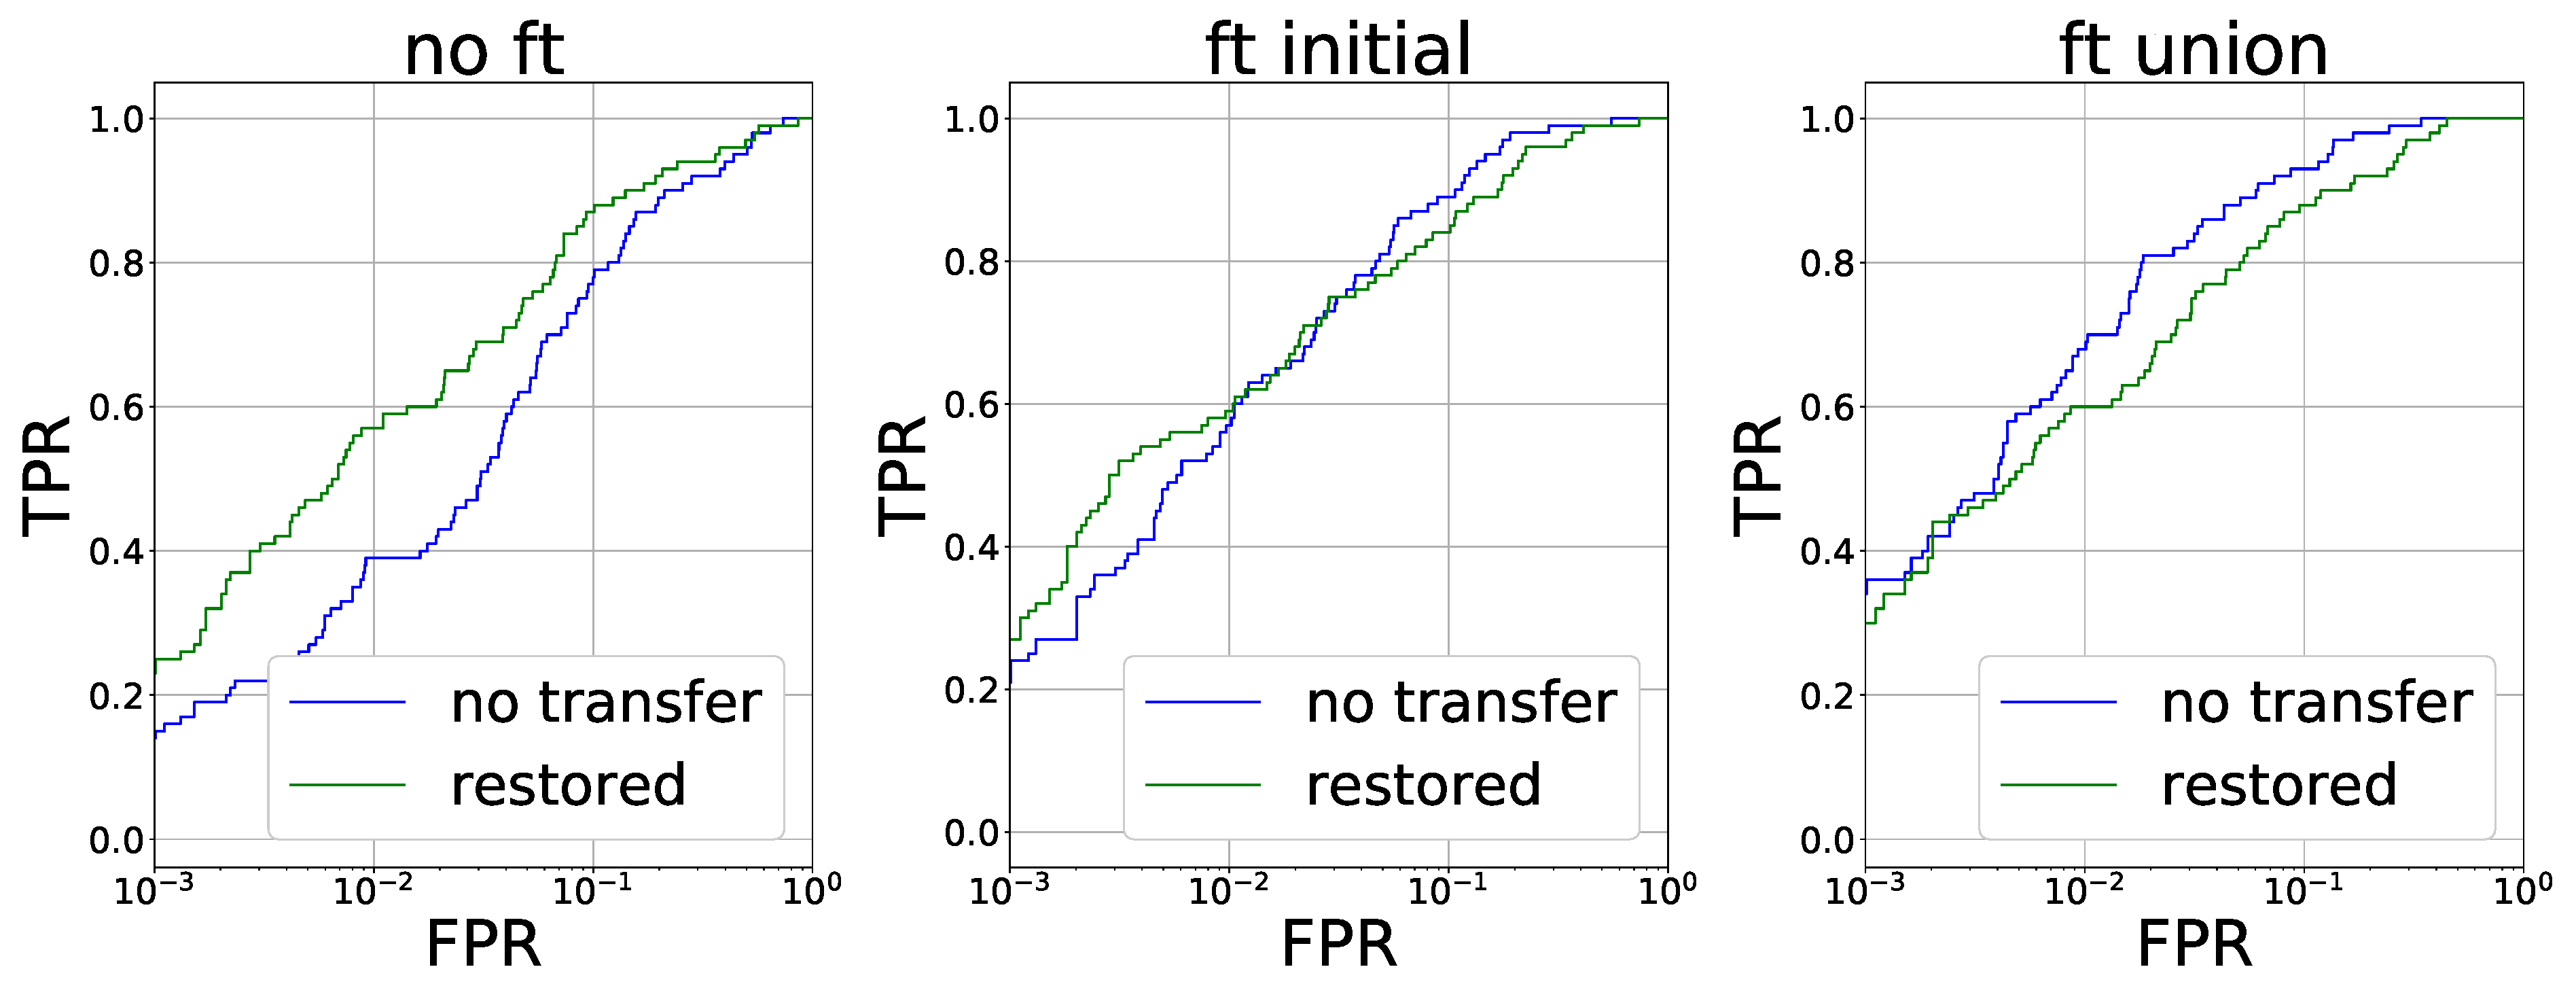
\includegraphics[width=\linewidth]{Chapters/face/Fig3.eps}
    \caption{The ROC curves for our face recognition models for different types of test data. Left -- \textit{no ft} model, test data transformation (the curve is denoted by 'restored') improves recognition. Middle -- \textit{ft initial}, the results for test data transformation are not clearly better than the results for initial images. Right -- \textit{ft union} model, the best results are for initial test data, without transformation. See \ref{sect:restoration_comparison} for the details. }\label{fig:roc_oxford_gan_vs_initial}
  \end{figure}

\bigskip\indent\textbf{Does restoration help recognition?} \\
%\subsubsection{Does restoration help recognition?}
\label{sect:restoration_comparison}
We start by assessing the improvement that the restoration process brings to the recognition. For this we evaluate the performance of the three different recognition networks discussed above, when they are applied either to untransformed surveillance-domain images or to surveillance-domain images transformed to the Internet image domain (using the learned mapping $F^{T \rightarrow S}$). See  \fig{lr_hr_gan_res_ytube_initial_degraded} for the example results of the Internet domain  transfer.

The ROC-curves in  \fig{roc_oxford_gan_vs_initial} shows that while the restoration process helps for the \textit{no ft} network, it actually \textit{hurts} for the better-performing \textit{ft initial} and \textit{ft union} networks. While trying to improve the results of the reverse transfer, we have also tried to transfer only the LR subset of the training images, while keeping the HR subset intact, but this lead to uniformly worse results.

We conclude that restoration does not necessarily help the recognition process in our setting. 



\begin{figure}
 \centering
    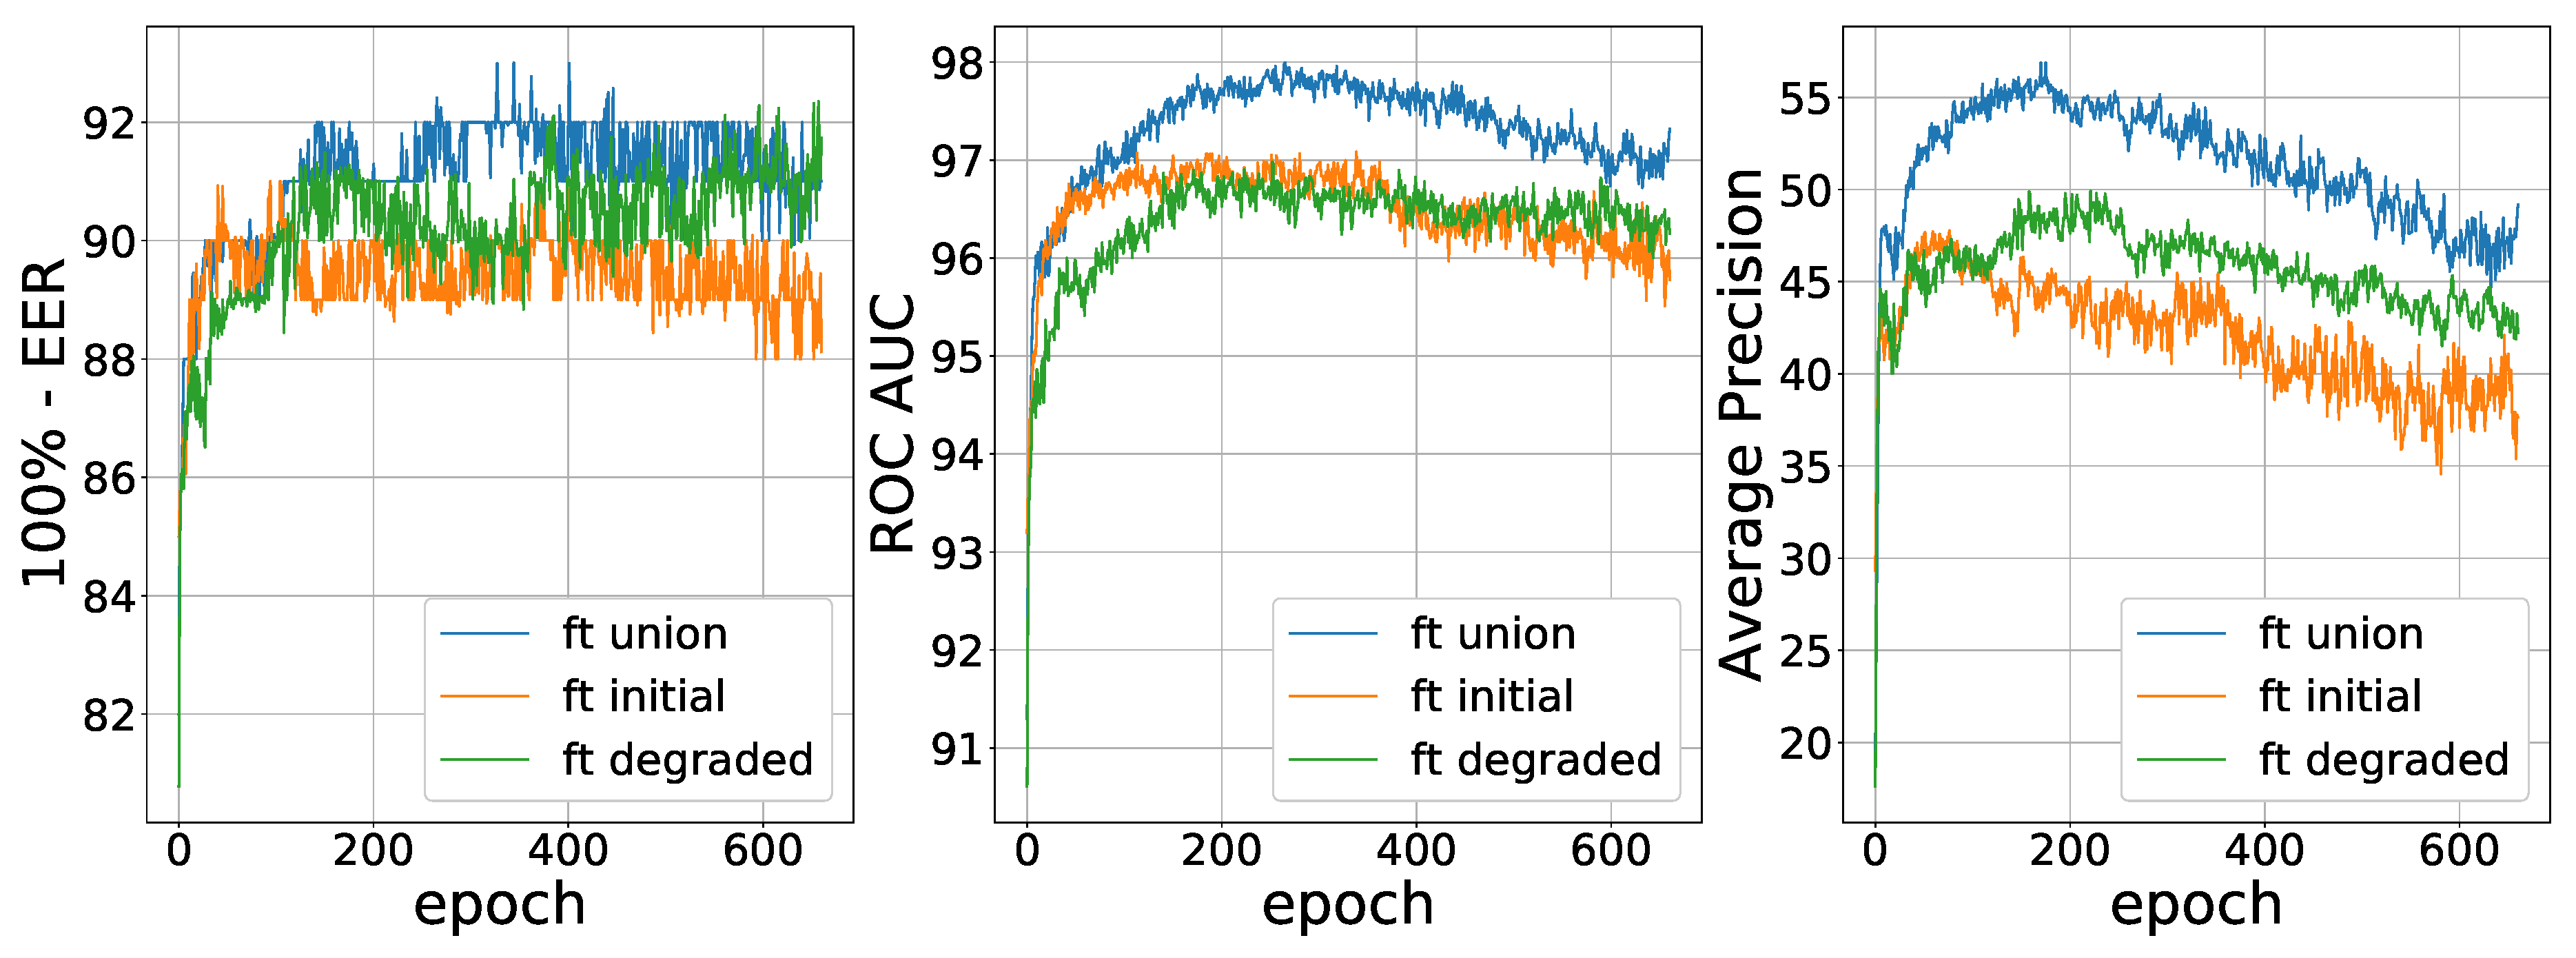
\includegraphics[width=\linewidth]{Chapters/face/Fig4.eps}
    \caption{The change of the recognition metrics for our surveillance validation set. \textit{ft degraded} and \textit{ft union} models that use our image-level domain adaptation overfit less than \textit{ft initial} that use only the initial Internet-domain data. The improvement is consistent across the two cases when VGG face and YTF datasets were used as Internet image data. See subsection \ref{sect:ft} for the models description.}\label{fig:validation_ytube}
  \end{figure}
  
  \begin{figure}

  \centering
    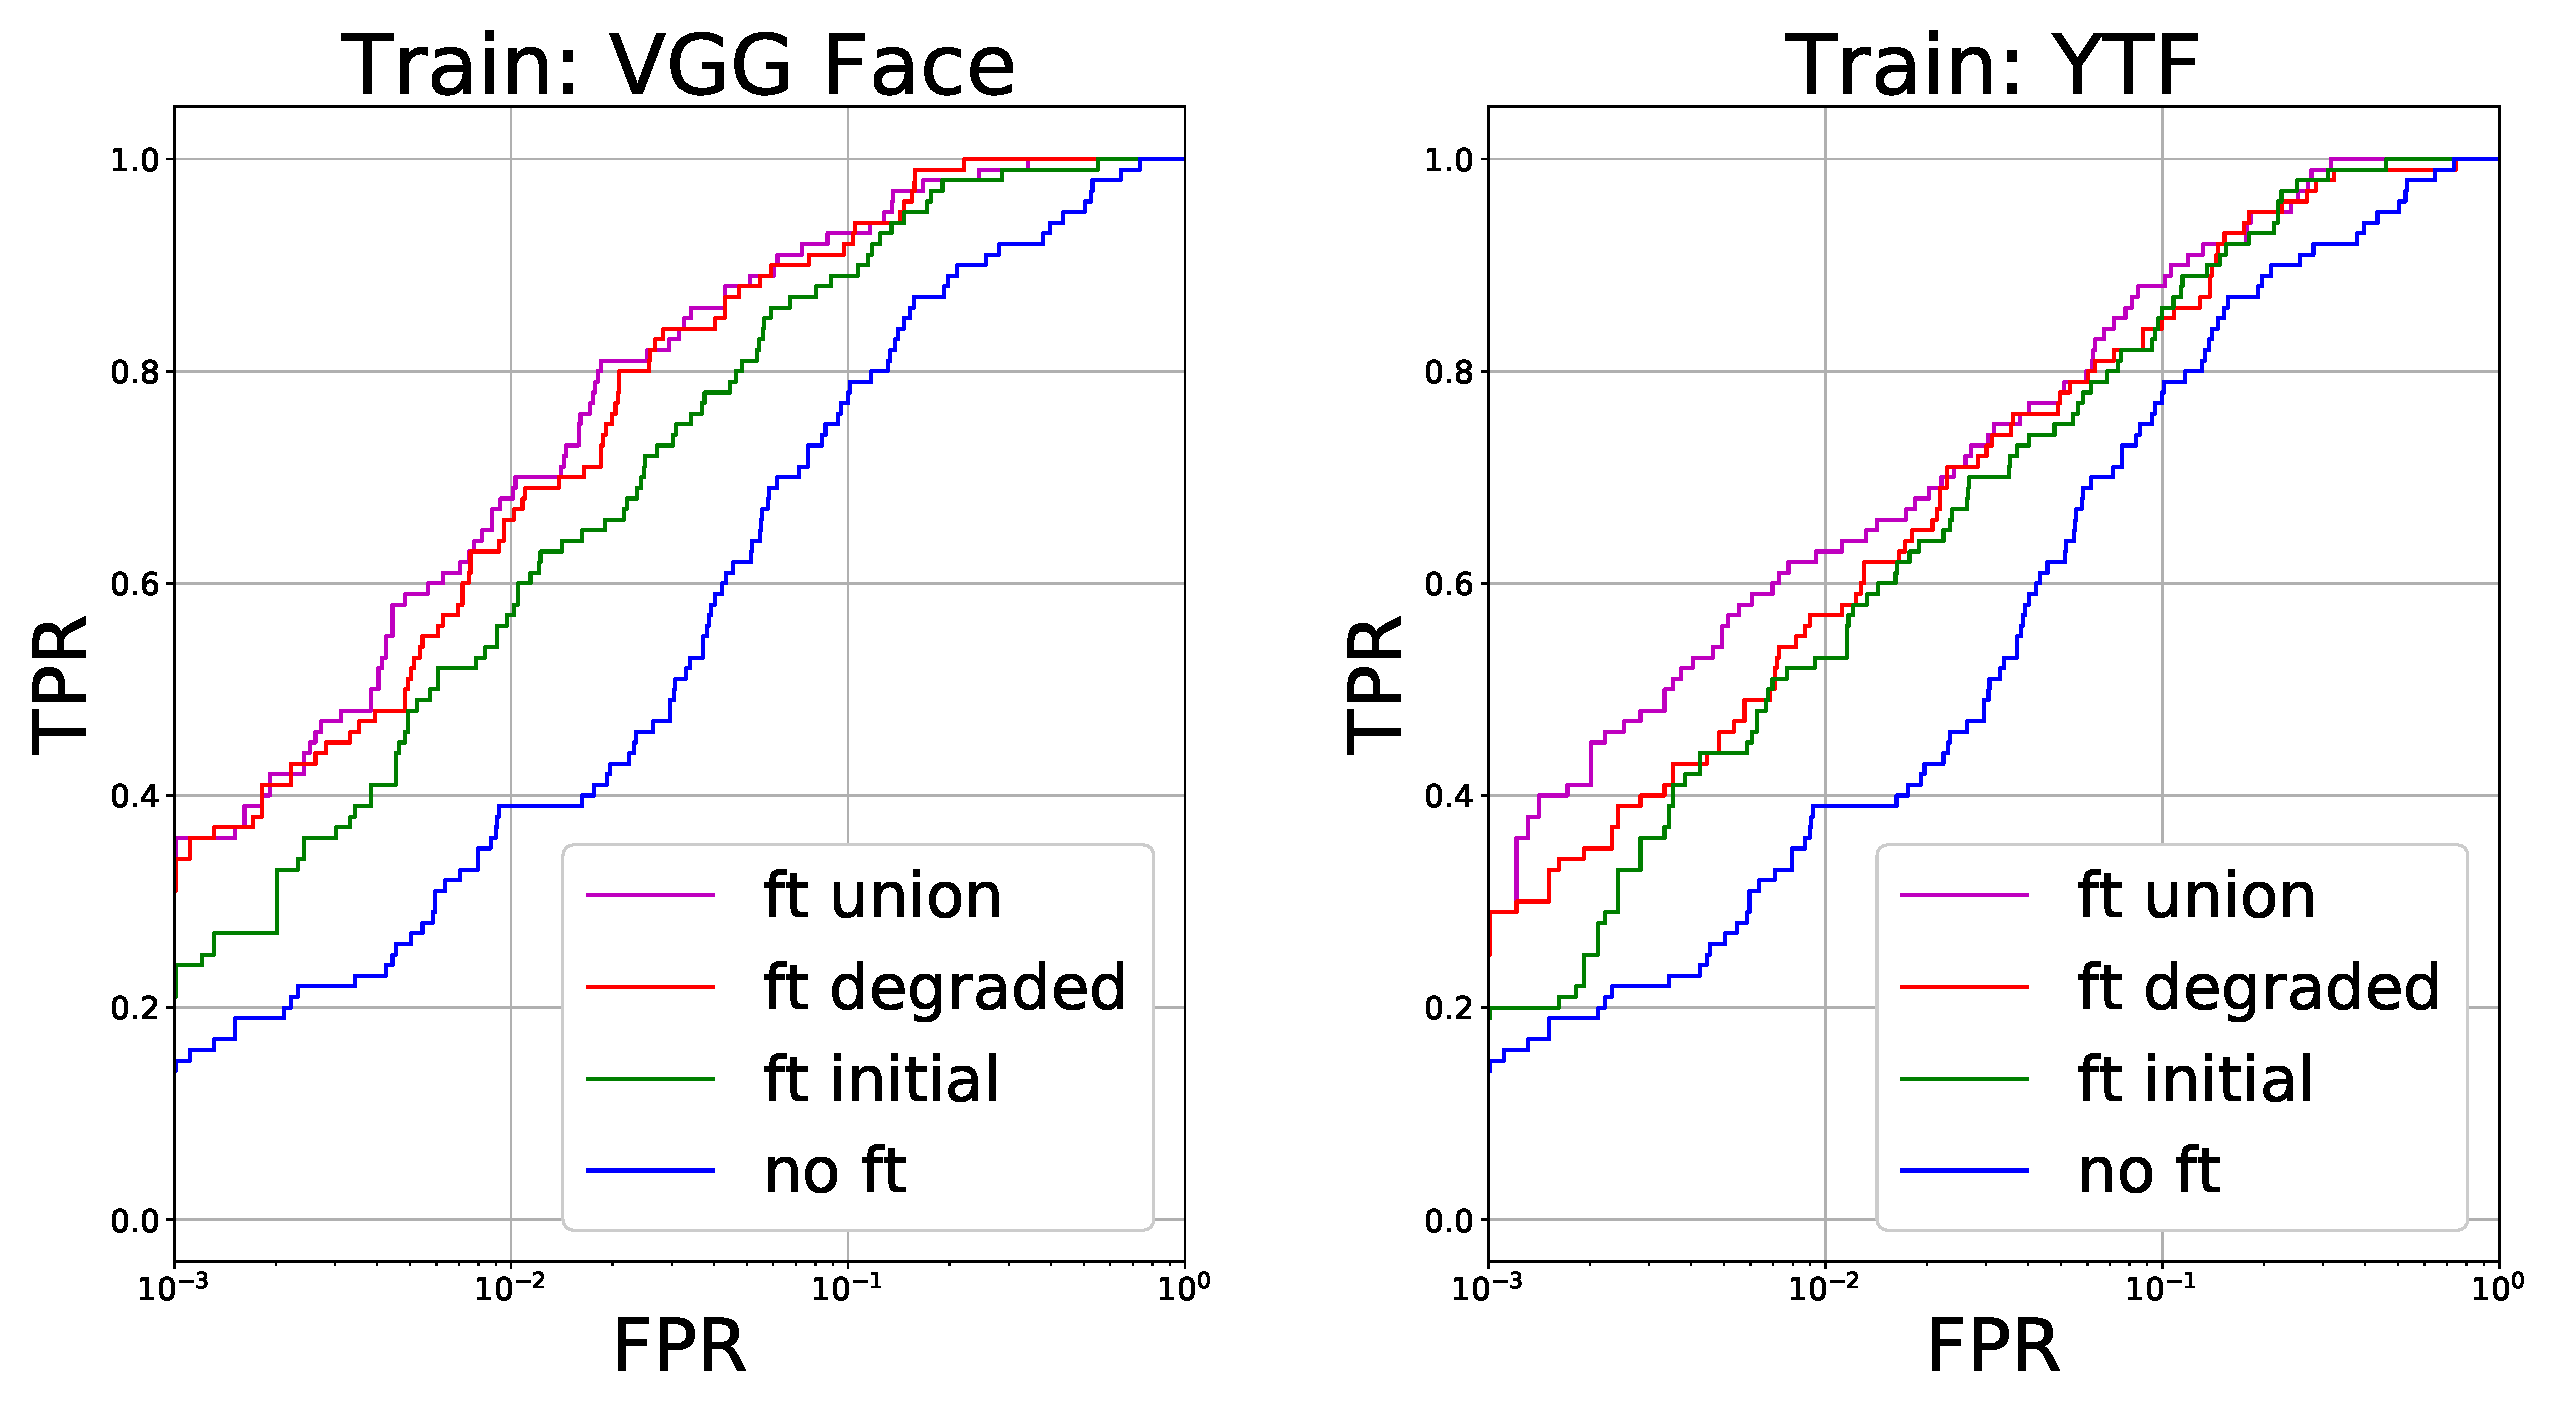
\includegraphics[width=\linewidth]{Chapters/face/Fig5.eps}
    \caption{The ROC curves for the fine-tuning strategies described in \sect{ft}. Our surveillance data is used for test. \textit{ft degraded} and \textit{ft union} models that use our image-level domain adaptation are better than other models. }\label{fig:roc_oxford_ytube}
  \end{figure}
  
 
\begin{table}
\flushbottom

\centering
\caption{Quality metrics for different face recognition models compared in this work (\ref{sect:ft}). The best model is \textit{ft union}, it is trained on both initial and degraded data.}
\label{tab:comparison}
\resizebox{\columnwidth}{!}{
\begin{tabular}{|c|c|c|c|c|c|c|}
\hline
\multicolumn{1}{|l|}{}   & \multicolumn{6}{c|}{Train datasets}                      \\ \hline
\multicolumn{1}{|l|}{}   & \multicolumn{3}{c|}{YTF} & \multicolumn{3}{c|}{VGG Face} \\ \hline
Fine-tuning type & 100\%$-$eer & roc auc & AP & 100\%$-$eer   & roc auc   & AP  \\ \hline
no ft                    &  84.73 & 91.52 & 25.98 &   84.73 & 91.52 & 25.98  \\ \hline
ft initial               &  88.52 & 95.67 & 42.38 &  89.32 & 96.62& 44.10  \\ \hline
ft degraded              &  87.03         & 95.53 &  47.02 & 90.28 &\bf{97.84} &53.33  \\ \hline
ft union                 &  \bf{89.41}    &   \bf{96.45} &\bf{50.91}&    \bf{91.31} &97.80 &\bf{54.89}   \\ \hline
\end{tabular}
}
\end{table}

  
 
%\subsubsection{Does domain adaptation help recognition?}
\bigskip\indent\textbf{Does domain adaptation help recognition?} \\
\label{sect:results}
We now consider the second scenario based on domain adaptation and thus compare the performance of different recognition networks described above on surveillance data. Our findings for image level domain adaptation are summarized in Table~\ref{tab:comparison}, which shows metric values for the compared training settings, and \fig{validation_ytube}, which shows validation metrics changes during training. Finally, \fig{roc_oxford_ytube} shows the final ROC curves.

The following can be observed. First, fine-tuning the VGG Face model on either VGG Face dataset or the YTF dataset using the BinDev loss (\textit{ft initial}) lead to a considerable improvement over the original state of the network.
Furthermore, we found that fine-tuning in the \textit{ft degraded} setting is clearly beneficial compared to \textit{ft initial} setting in the case of the VGG Face training dataset, and a little bit better for the YTF training data, overall making a case for image-level domain adaptation. The results of the \textit{ft union} setting are uniformly better than \textit{ft initial} and \textit{ft degraded} suggesting that the automatically degraded data are a useful augmentation, but that the original data should not be discarded. 
Finally, \fig{tsne} gives an additional evidence of the success of domain adaptation. It shows that the feature distribution of our surveillance data is more intermixed with those of the degraded version of the YTF dataset than its initial version. This demonstrates the relevance of the suggested augmentation (via image-level domain adaptation).



% \subsubsection{Comparison to the reverse domain transfer}
% \label{sect:restoration_comparison}

% We have also investigated the restoration-based approach (\sect{strategies}), using the reverse mapping $F^{S \rightarrow T}$ that also comes out as the result of training the model \ref{sect:domain_transfer}. 
% Here we test our previously trained face recognition models (described in  \sect{ft}) on different variants of test data. See  \fig{lr_hr_gan_res_ytube_initial_degraded} for the example results of the Internet domain  transfer.

% We have evaluated the effect of such reverse transfer to the higher-quality domain at test term for the \textit{no ft}, \textit{ft initial}, and \textit{ft union} networks described in the previous subsection. The ROC-curves in  \fig{roc_oxford_gan_vs_initial} shows that while the reverse transfer helps for the \textit{no ft} network, it actually hurts for the better working \textit{ft initial} and \textit{ft union} networks. While trying to improve the results of the reverse transfer, we have also tried to transfer only the LR subset of the training images, while keeping the HR subset intact, but this lead to uniformly worse results.

%in the case of the pre-trained VGG face network (\textit{no-ft}), transferring low-quality test images into the Internet data domain improves recognition. Nevertheless, if we use one of the fine-tuned models for recognition, the results for the initial test images are not worse than those for transferred images. Moreover, ROC curve for initial test images is the highest for our best \textit{ft union} model as shown in \ref{fig:roc_oxford_gan_vs_initial}-right.



%\subsubsection{Comparison to feature-level domain adaptation}

\bigskip\indent\textbf{Comparison to feature-level domain adaptation} \\
\label{sect:grl}
We have additionally compared our image-level domain adaptation (all the experiments and discussions above) to the feature-level domain-adversarial adaptation approach described in \chapt{gradrev}. Tuning this approach required some effort (several modifications from the settings of \chapt{gradrev} were needed to make such adaptation work). We thus built a DANN (Deep Adversarial Neural Network) based on the VGG-face network. The  domain classifier consists of three fully-connected layers: $512$ units in the first two layers (Leaky ReLU \cite{HeZRS15} non-linearities were used) and one classification layer with $1$ unit. Dropout with $0.5$ probability was inserted before the classification layer. The Gradient Reversal layer is attached after the \textit{fc6} layer of VGG-face. We found that schedule for the adaptation parameter  $\lambda$ is very important for this task. Instead of the schedule suggested in \chapt{gradrev} (which did not lead to good results in our comparison), we set $\lambda$ to $1e-3$ for the first $20$ epochs and then increased it to $1e-2$. 

Using the scheme described above when training on the VGG Face dataset, we have achieved the following results: $100$\% - EER was $88.64$, ROC AUC was $96.69$ and the average precision was $52.11$. This is better than the results of our \textit{ft initial} setting, but worse than those of \textit{ft degraded} and \textit{ft union} settings (for the last, the results are $91.31$, $97.80$ and $54.89$ correspondingly). Other setting for feature-level domain adaptation that we have tried lead to worse results.






  
  
  
  


 

  \begin{figure}
  \centering
    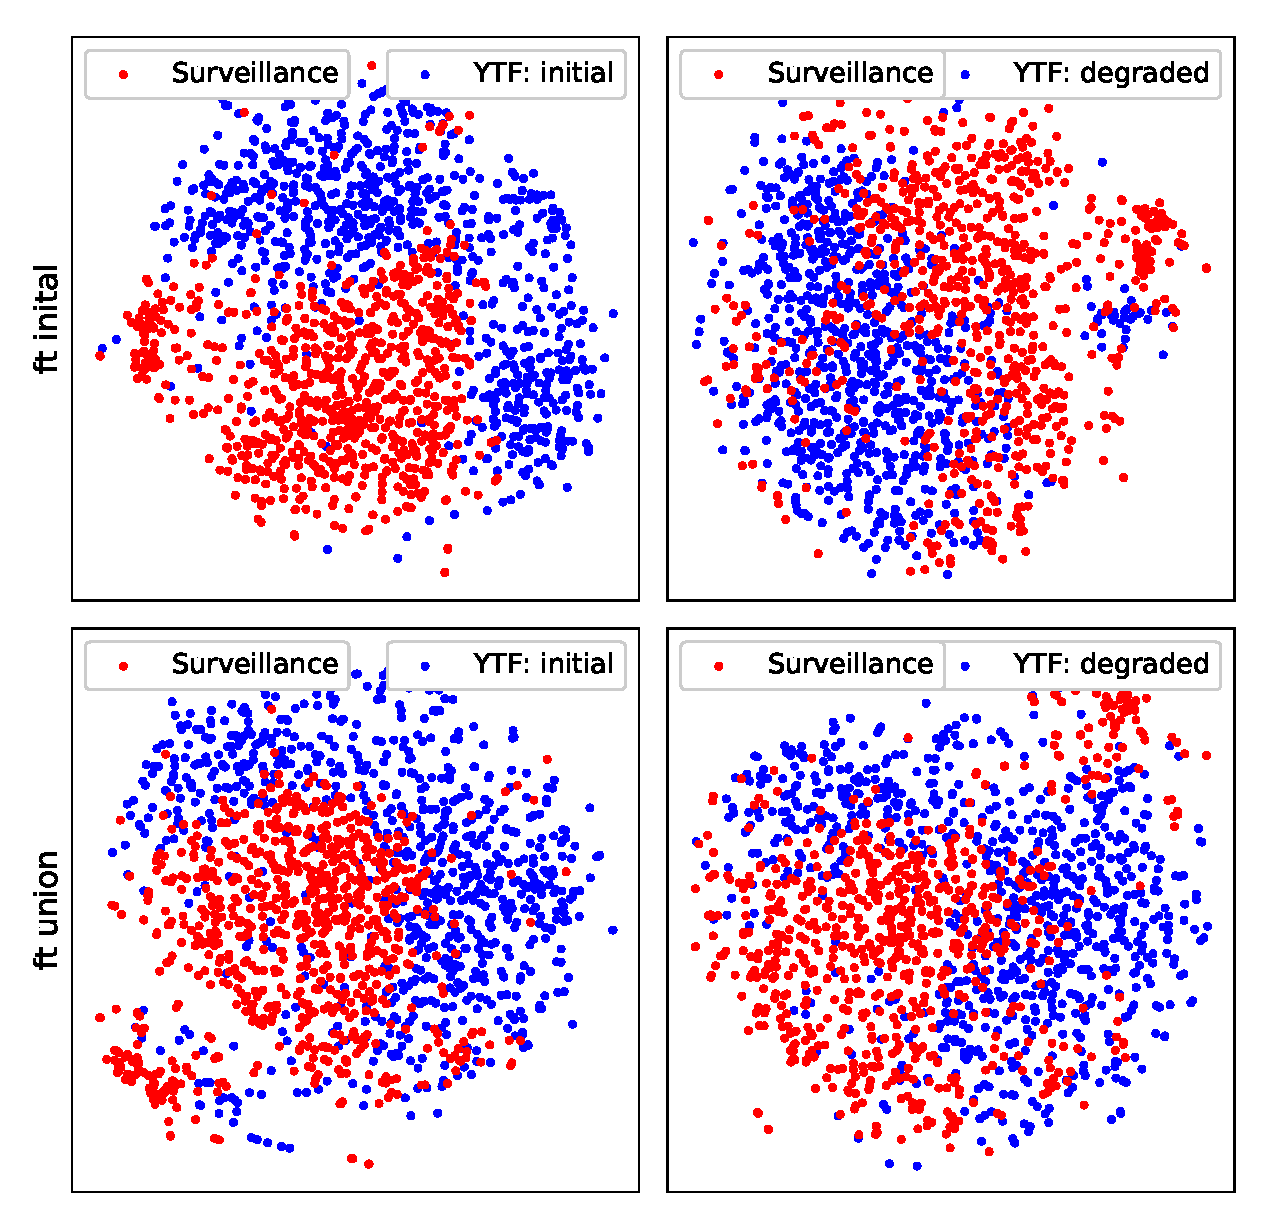
\includegraphics[width=\linewidth]{Chapters/face/Fig6.eps}
    \caption{t-SNE \cite{maaten2008visualizing} visualizations for deep features extracted with: first row -- \textit{ft initial}, second row -- \textit{ft union} neural nets (See \ref{sect:ft} for the descriptions of the models). For both nets, surveillance data distribution is more intermixed with the degraded version of the YTF dataset than with its initial version.}\label{fig:tsne}
  \end{figure}


\section{Conclusion}
\label{sect:conclusion}

% Discuss your conclusions in order of most to least important.

In this chapter, we have compared the image-based domain adaptation techniques for face recognition in the presence of strong image degradation. We consider the recently proposed CycleGAN approach for learning mappings between the two domains of surveillance data and Internet face images. We demonstrate that the strategy of transferring the labeled Internet data to the surveillance domain and subsequent retraining the face recognition network helps to improve the recognition quality on real surveillance test data. We have investigated the variants of this approach, and have demonstrated that training on both transferred and original Internet data leads to the optimal performance. Finally, we show that in the case of our domain pair, the image-level adaptation approach outperforms feature-level domain adaptation. 

%Compare your results with those from other studies: Are they consistent? If not, discuss possible reasons for the difference.
We found our results consistent with \cite{SohnLZY0C17}, where face recognition for the low-quality is also considered. In \cite{SohnLZY0C17},  verification accuracy was improved using carefully chosen data augmentation. It is an interesting fact, that the improvement remained noticeable even when the data augmentation and the feature-level domain adaptation were applied simultaneously. Here, in contrast, we suggest performing the data augmentation in a more automatic way. Although we do not experiment with the combination of feature-level and image-level approaches to domain adaptation, we compare them independently. The combination of these adaptation techniques may further improve the results.


% Mention any inconclusive results and explain them as best you can. You may suggest additional experiments needed to clarify your results.
In our experiments, best results were achieved with training on both domains. An explanation can be given that the domain transfer model is imperfect and may push different images of the same identity too far as we do not use any kind of verification loss for training (ideally, this would require another pre-trained network for the low-quality domain, which essentially is the goal of this work). Therefore, keeping the initial data in the training set may result in less overfitting. %This can be explained by the fact that our target domain is not uniform in terms of data quality. We use two parts of the same track to generate matching pairs for each identity: e.g. these parts of each track differ in resolution (see \ref{fig:lr_hr_gan_res_ytube_initial_degraded}, columns $1$ and $3$). Therefore, using training data of diverse quality may lead to better results.  -- not true, checked.

% Briefly describe the limitations of your study to show reviewers and readers that you have considered your experiment’s weaknesses. Many researchers are hesitant to do this as they feel it highlights the weaknesses in their research to the editor and reviewer. However doing this actually makes a positive impression of your paper as it makes it clear that you have an in depth understanding of your topic and can think objectively of your research.

As an important negative result, we show that using CycleGAN-based restoration of lower-quality domain images by transferring them to the higher-quality domain does not bring consistent improvement to the recognition performance. We speculate that such transfer may distort some details of the images in a non-identity preserving way.

Our study considers a practically important domain of image data. 
We note, however, that our findings might not transfer to other pairs of domains in image adaptation.


% Discuss what your results may mean for researchers in the same field as you, researchers in other fields, and the general public. How could your findings be applied?
 
% State how your results extend the findings of previous studies.
% If your findings are preliminary, suggest future studies that need to be carried out.
% At the end of your Discussion and Conclusions sections, state your main conclusions once again.


\textbf{Acknowledgement:}  This research is supported by VisionLabs and the Ministry of Education and Science of the Russian Federation (grant 14.756.31.0001). 

% \appendix
% \section{Feature-level domain adaptation settings}
% \label{sect:app_grl}
% Here we describe the settings for the feature-level domain adaptation (used in the comparison of Section~ \ref{sect:grl}). We built a DANN (Deep Adversarial Neural Network) based on the VGG-face network. The  domain classifier consists of three fully-connected layers: $512$ units in the first two layers (Leaky ReLU \cite{HeZRS15} non-linearities were used) and one classification layer with $1$ unit. Dropout with $0.5$ probability was inserted before the classification layer. The Gradient Reversal layer is attached after the \textit{fc6} layer of VGG-face. We found that schedule for the adaptation parameter \lamdba is very important for this task. Instead of the schedule suggested in \cite{GaninUAGLLML16} (which did not lead to good results in our comparison), we set \labmda to $1e-3$ for the first $20$ epochs and then increased it to $1e-2$. 




%\begin{acknowledgements}
%If you'd like to thank anyone, place your comments here
%and remove the percent signs.
%\end{acknowledgements}

% BibTeX users please use one of
%\bibliographystyle{spbasic}      % basic style, author-year citations
%\bibliographystyle{spmpsci}      % mathematics and physical sciences
%\bibliographystyle{spphys}       % APS-like style for physics

%\bibliography{main}


% end of file template.tex

